Frequent patterns are structures that occur frequently in a data set. We want to find inherent regularities. 

An important part of frequent pattern mining is the \textbf{Downward closure property}, or the A priori principle. It states that any item that contains $X$ also contains a subset of $X$. So if we already have verified that $X$ is infrequent, then the supersets must be infrequent.

By our definition, a (sub)graph is frequent if its support (Occurrence frequency) in a dataset is no less than a minimum support threshold. 

Unfortunately, there are an exponential number of patterns in graphs. This means that we have to a number of different approaches, such as pattern-growth approaches, or Apriori-based approaches. 

Apriori approaches start with a small-sized subgraph and proceeds in a bottom-up manner. Patterns are then joined to create bigger patterns through the Apriori principle. Pattern-growth approaches extends existing frequent subgraphs by adding edges at a time.

\subsection{Frequent subgraph mining on graph collections}
    We define support as the frequency of a subgraph appearing in a set of graphs. The Apriori principle for graphs is that if a graph is frequent, then all of its subgraphs are frequent. 
    
    The \textbf{Subgraph Mining problem} is as follows 
    \begin{itemize}
        \item Given a set of labeled graphs $D = \set{G_1, G_2, \dots, G_n}, G_i = \langle V_i, E_i, l_i \rangle$ and a subgraph $G$, the supporting set of $G$ is $D_G = \set{G_i | G \sqsubseteq G_i, G_I \in D}$ where $G \sqsubseteq G_i$ indicates that $G$ is a subgraph isomorphic to $G_i$
        \item The support is $\sigma(G) = \frac{|D_G|}{|D|}$
        \item The input is a set of labeled graphs $D = \set{G_1, G_2, \dots, G_n}$, $G_i = \langle V_i, E_i, l_i$. And the minimum support minsup
        \item It outputs if a subgraph $G$ if $\sigma(G) \geq $ minsup, and if each subgraph is connected. 
    \end{itemize}
    Note that support is anti-monotone for all $G' \sqsubseteq G, \sigma(G') \geq \sigma(G)$. 
    
 \subsection{Apriori-based approaches (FSG)}
    Notation goes as follows: $k$-subgraph is a subgraph with $k$-edges. We initialize by scanning the transactions to find $F_1$, the set of all frequent $1$-subgraphs with counts, and all $2$-subgraphs with counts. The algorithm proceeds as follows:
    \begin{enumerate}
        \item For $k=3, F_{k-1} \neq \emptyset, k++$
        \item \textbf{Candidate generation:} Get $C_k$, the set of candidate $k$-subgraphs from $F_{k-1}$, the set of frequent $(k-1)$-subgraphs. 
        \item \textbf{Candidate pruning:} For a candidate to be frequent, each $(k-1)$ subgraph should be frequent
        \item \textbf{Frequency pruning:} Scan database, count occurrences of subgraphs in $C_k$
        \item $F_k = \set{c \in C_k | c  \text{has counts no less than minsup}}$ 
        \item Return $F_1 \cup \dots \cup F_k$
    \end{enumerate}
    In candidate generation, we need to determine graph isomorphisms to determine candidates to join, to check downward closure, we need graph isomorphism, and to check containment of a frequent subgraph, we need subgraph isomorphism. This is NP-hard. 
    
    We can do the following
    \begin{itemize}
        \item Candidate generation: Use core detection. (Subgraphs may have the same core) \footnote{Elaborate on core detection}. We build $k$-subgraphs from $k-1$ subgraphs, so the core remains the same, but we expand them
        \item Candidate pruning: Use canonical labeling 
        \item frequency counting: Use TID Lists
    \end{itemize}
    
    For candidate pruning, we can construct a canonical labeling based on the adjacency matrix. We concat the columns (if undirected only upper right matrix). The canonical code is then $Code(G) = \min{code(M) | M \text{is adjacency matrix}}$. We can then ask if two subgraphs are the same by checking their codes. This way we can check if a subgraph is frequent by comparing them against hashes of frequent subgraphs. Finding a canonical labeling is as complex as graph isomorphism, but we have heuristics such as vertex invariants, neighbor lists and iterative partioning to speed it up. 

    For frequency counting, we can use the following idea. For each pattern $f_1, \dots, f_r$. We take a list of graph TIDs that contain the pattern. When joining two patterns compute intersection between lists. If size of intersection is smaller than min support, then get rid of that pattern. For example, $G_1 = \set{f_1, f_2, f_3}, G_2 = \set{f_1}, G_3 = \set{f_2}$, then $TID(f_1) = \set{G_1, G_2}, TID(f_2) = \set{G_1, G_3}$, then for a candidate $c = join(f_1, f_2)$, we say that $TID(C) = \text{subset of TID}(f_1) \cap TID(f_2)$. The need to check isomorphism does not arise with frequent itemsets. 
    
    These approaches are simpler for some graphs, but in general still NP hard.
    
\subsubsection{Pattern-growth approaches (gSPAN)}
    It uses properties of DFS traversals to define canonical codes. Reduces reduncancy in pattern generation. 
    
    We will use a \emph{prefix tree}, that is a canonical representation of itemsets obtained by a complete order over the items. Each possible itemset appears in the tree exactly once. The properties of a tree search space is that for each $k$-label, its parent is the $k-1$ prefix of the given $k$-label. The relation among siblings is an ascending lexicographic order.
    
    We map a graph to a sequential DFS code for a certain DFS traversal. We will construct lexicographically ordered codes and construct tree search space based on the lexicographic order. 

    \begin{center}
        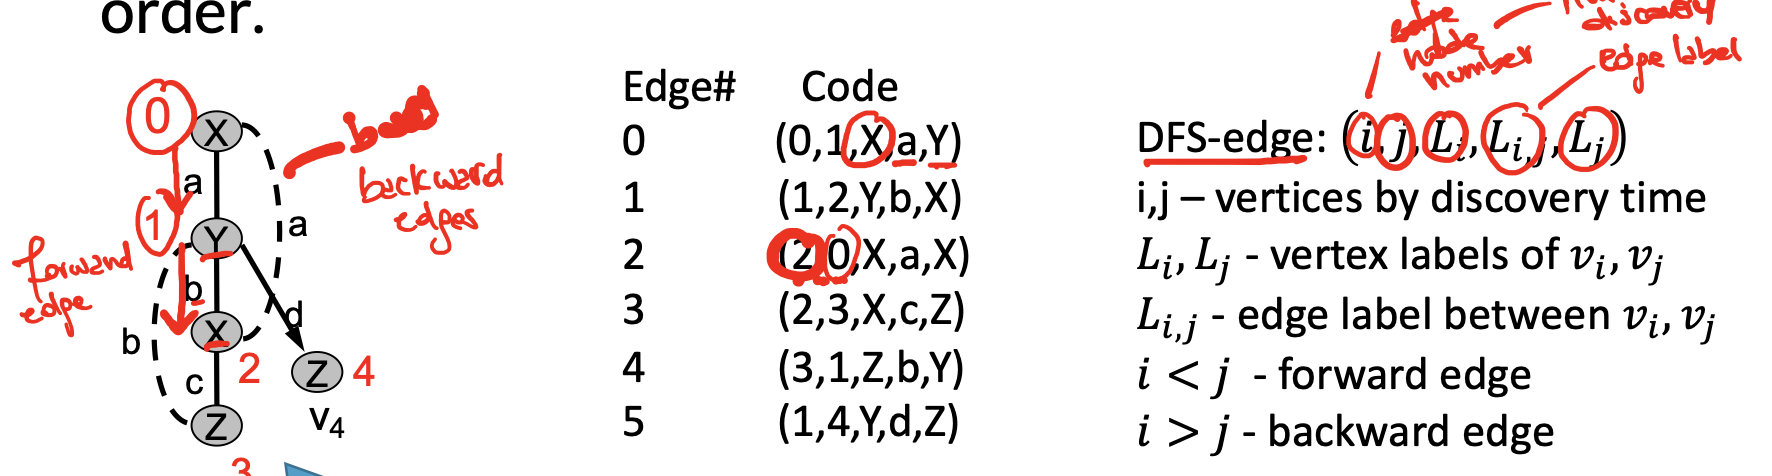
\includegraphics[width=1\textwidth]{images/dfs1.png}
    \end{center}
        \begin{center}
        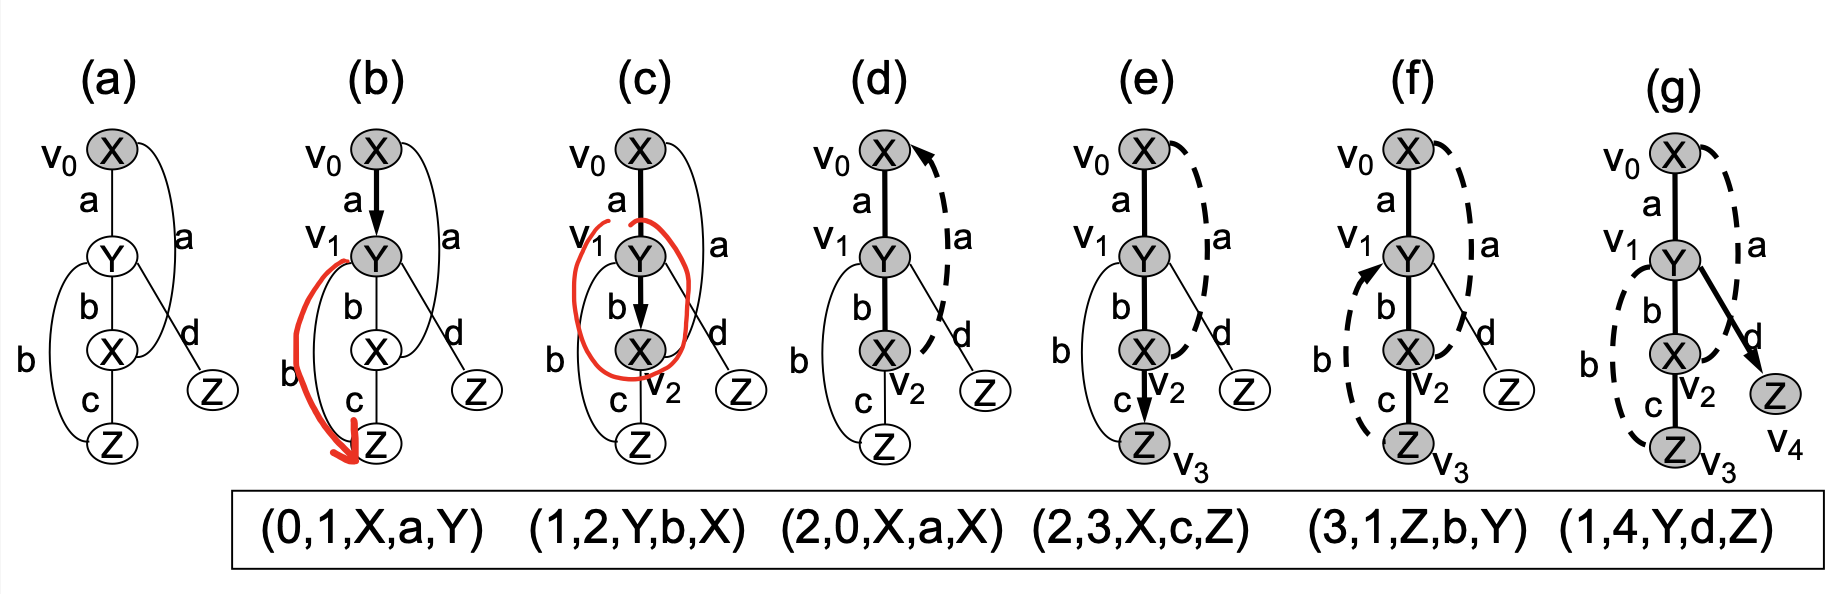
\includegraphics[width=1\textwidth]{images/dfs2.png}
    \end{center}
    
    We define a specific order on edges corresponding to the DFS traversal. The rules for the code is
    \begin{itemize}
        \item $e_n = (i_n, j_n)$ 
        \item $e_1 \prec e_2 \implies e_1$ appears before $e_2$ in the code
        \item If $i_1 = i_2$ and $j_1 < j_2 \implies e_1 \prec e_2$ 
        \item $i_1 < j_1$ and $j_1 = i_2 \implies e_1 \prec e_2$
        \item If $e_1 \prec e_2$ and $e_2 \prec e_3 \implies e_1 \prec e_3$
    \end{itemize}
    
    We do not want multiple codes for the same graph, so we need a unique representation. We define a total order so we can find the minimum. If two minimum codes are the same, then the graphs should be isomorphic. 
    
    The ordering is 
    \begin{itemize}
        \item Let $\alpha = (a_0, a_1, \dots a_m), \beta = (b_0, b_1, \dots, b_n)$
        \item $\alpha \leq \beta$ iff either are true
        \item $\exists t, 0 \leq t \leq min(n, m)$ such that $a_k = b_k$ for $k < t$ and $a_t \prec_e b_t$
        \item Or $a_k = b_k$ for $0 \leq k \leq m$ and $n \geq m$
    \end{itemize}
    
    Let us now define precende among DFS codes
    
    \begin{itemize}
        \item $a_t = (i_a, j_a, L_{i_a}, L_{i_a, j_a}, L_{j_a})$
        \item $b_t = (i_b, j_b, L_{i_b}, L_{i_b, j_b}, L_{j_b})$
        \item Then $a_t \prec _bt$ if 
        \begin{enumerate}
            \item Both are forward edges (hence both arrive at new node indexed as $j_a = j_b)$ and \begin{itemize}
                \item $i_b < i_a$ (edge starts from later visited vertex) OR
                \item $i_b = i_a$ and the labels of $a$ are lexicographically less than labels of $b$ in order of tuple
            \end{itemize}
            \item Both are backward edges (hence both start from node indexed as $i_a = i_b$ and
            \begin{itemize}
                \item $j_a < j_b$ (edge connected to an earlier discovered vertex) OR
                \item $j_a = j_b$ and edge label of $a$ is lexicographically less than the one of $b$
            \end{itemize}
            \item $a_t$ is backward and $b_t$ is forward
        \end{enumerate}
    \end{itemize}
    
    The parent-child relation is that if $\min(G_1) = \set{a_0, a_1, \dots, a_n}$ and $\min(G_2) = \set{a_0, a_1, \dots, a_n, b)}$ that is prefixes, then $G_1$ is parent of $G_2$. A valid DFS requires that $b$ (which by definition is larger than any $a_i$ grows from a vertex on the rightmost path. If it is not in the rightmost path, then it has already been discovered by DFS.
    
    For \textbf{Subgraph search space (DFS Tree)}, we can organize DFS codes by parent-child rules. An in-order traversal follows DFS lexicographic order.
    
    The gSpan algorithm is as follows:
    \begin{itemize}
        \item We want to traverse DFS-code tree for a given label sets, then prune using support, minimality of codes. It outputs frequent subgraph set $S$
        \item \begin{enumerate}
            \item Let $S$ be frequent one-edge subgraphs in $D$ using DFS code.
            \item Sort $S$ in lexicographic order
            \item $N = S$
            \item For each $n \in N$, $gSpanExtend(D; n, minsup, S)$
            \item Strategy: Grow minimal DFS that occur frequently in $D$.
        \end{enumerate}
    \end{itemize}
    The GspanExtend works as follows
    \begin{itemize}
        \item If $n$ not minimal (expensive) end
        \item Otherwise, add $n$ to $S$, for each single-edge rightmost expansion $e$ of $n$: 
        \begin{itemize}
            \item if $\sigma(e) \geq minsup$, then $gspanextend(D, e, minsup, S)$
            \item Remove $n$ from all graphs in $D$ (Consider only subgraphs not already enumerated)
        \end{itemize}
    \end{itemize}
    
\subsection{Greedy approach (Subdue)}
    We consider a greedy algorithm that finds some of the most prevalent subgraphs. It is not complete, and is based on the minimum description principle. It uses patterns that give maximum compression. It uses Beam Search, and like BFS it progress level by level. Unlike BFS, beam search only moves downward through the best width nodes at each level.
    
\subsection{Frequent subgraph mining on a single graph}
    Any support measure is admissible if for any pattern $P$ and any sub-pattern $Q \sqsubseteq P$, the support of $P$ is not larger than the support of $Q$. That is, we have the anti-monotonicity property. The number of occurrences of a pattern is not admissible. A number of admissible patterns are 
    
    \begin{itemize}
        \item Maximum independent set support (MIS): Based on maximum number of non-overlapping matches
        \item Harmful overlap support (HO): Based on number of patterns for which no multi-node subgraph is identical
        \item Minimum image-based support (MNI): Based on the number of times a node in the pattern is mapped into a distinct node in the graph
    \end{itemize}
    
    MIS is counting how many times a pattern is mapped to a non-overlapping subgraph. This is NP-hard. We can compute it with an \emph{overlap graph}, which is a graph that has an edge among each pair of overlapping matches. 
    
    Less restrictive is HO, which instead of considering overlap among single nodes considers harmful embeddings that share a common multi-node subgraph. 
    
    \begin{center}
        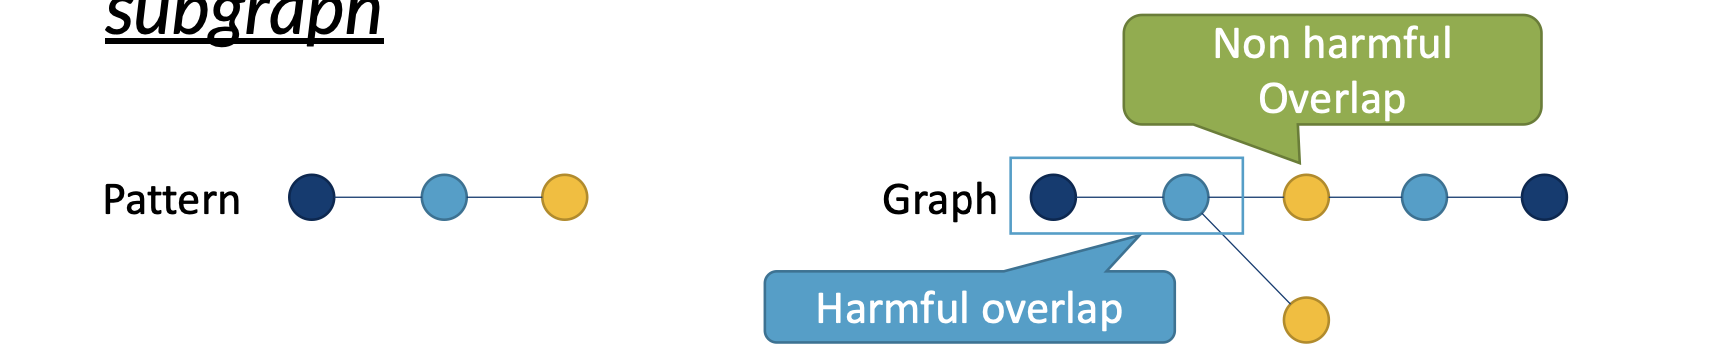
\includegraphics[width=1\textwidth]{images/HO.png}
    \end{center}
    
    MNI is simpler and considers (the minimum) number of times a node of the pattern is mapped to the graph. 
    
    \begin{center}
        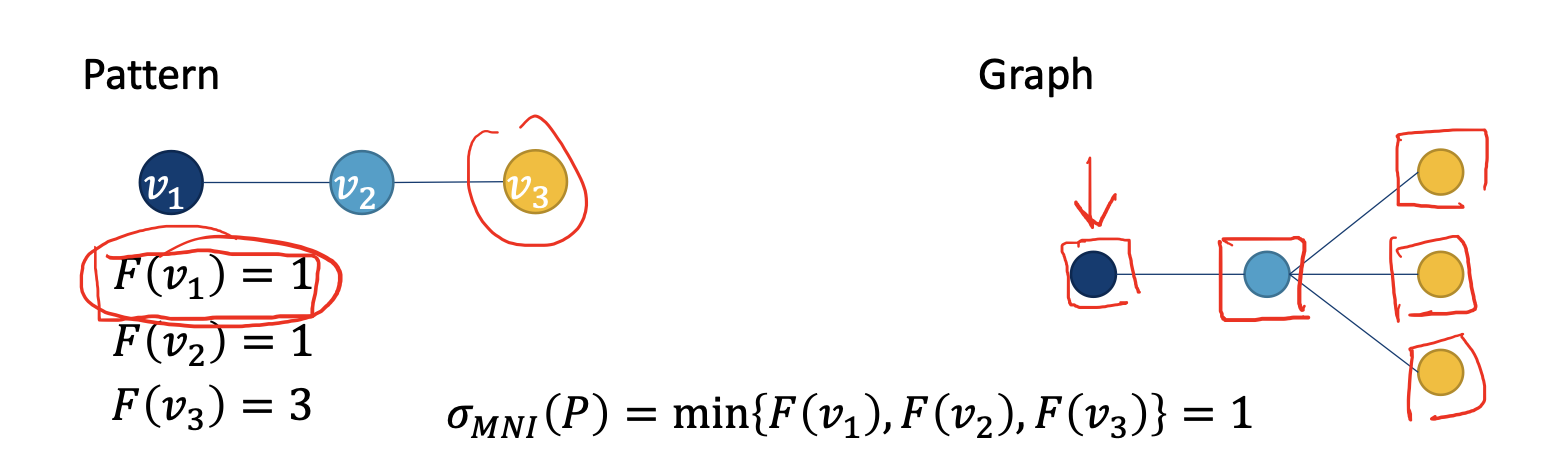
\includegraphics[width=1\textwidth]{images/minmatch.png}
    \end{center}
    
    MNI can be computed in polynomial time, the rest are NP hard.
    
    With an anti-monotone support measure, we can apply any previous support measure (such as gSPAN) just changing how the support is computed and leaving the rest unchanged. 
    
    We can use the grow and store approach to finding frequent subgraphs
    
    \begin{itemize}
        \item Add all frequent edges to the list of frequent subgraphs
        \item Extend frequent subgraphs to larger candidates
        \item Compute candidate frequency (find all occurrences)
        \item Repeat step 2 until no more frequent subgraphs is found
    \end{itemize}
    
\subsubsection{GraMi (solving gSpan)}
    gSpan may have excessive store requirements and slow performance. Here we map it to a variable assignment problem. 
    
\subsection{Mining frequent itemsets (The Apriori algorithm)}
    We want to find combinations of items that occur frequently. The support of an item is the number of sets in which it occurs. Brute force algorithms have to search through an exponential number of possible combinations, so we have to be clever about it. Here we can use the A-priori principle. If an itemset is frequent, so are its subsets. If an itemset is not frequent, so are its supersets. Support is anti-monotone, so the support of an itemset never exceeds support of subset. We can use the Apriori algorithm. It is split into two parts: \textbf{Frequent itemset generation}, and \textbf{candidate generation}.
    
    
    Let $C_k$ be the candidate itemsets of size $k$, let $L_k$ be the frequent itemsets of size $k$. Let $k = 1$ and $C_1$ be all items, then we do the following
    \begin{enumerate}
        \item Scan DB to find which itemsets in $C_k$ are frequent, put them into $L_k$
        \item Use $L_k$ to generate a collection of candidate itemsets $C_{k+1}$ of size $k+1$
        \item Repeat while $C_k$ is not empty
    \end{enumerate}
    The idea here is to combine frequent items into larger and larger itemsets considering only frequent building blocks.
    
    \subsubsection{Candidate generation}
        We will construct candidate sets of size $k+1$ by combining sets of size $k$. We assume that all itemsets are ordered, such as lexicographically. We also assume that itemsets in $L_k$ are also listed in order.
        \begin{itemize}
            \item If $k=1$, take all pairs of frequent items, if $k > 1$, combine pairs of itemsets that \emph{differ by one item}
            \item For each candidate itemset, check if all subsets of size $k$ are frequent.
            \item \textbf{Pruning step:} For each candidate $(k+1)$ itemset, create all $k$-itemsets. Remove a candidate if a $k$ subset is not frequent. 
        \end{itemize}
    
    The factors affecting complexity are 
    \begin{itemize}
        \item Minimum support threshold (the lower the more we have to deal with)
        \item Dimensionality of the dataset
        \item Size of Database (since Apriori makes multiple passes)
        \item Average transaction width. It may increase max length of frequent itemsets and traversals of hash tree
    \end{itemize}
    
    \subsubsection{Counting support}
        We use hashing to count the support of each itemset. We will use a hash tree structure in order to avoid excessive memory overhead, where we on the $i$-th level we hash the $i$-th item. The hash-tree also enables enumeration of itemsets in transaction and matching them against candidates. 
        
        We can also use a triangular matrix approach. \footnote{Elaborate on these}
        
    \subsection{Association rule mining (Apriori)}
        Given a set of transactions, find rules that predict the occurrence of an item based on occurrences of other items. Here implication means co-occurrence, not causality. For example, $\set{A, B} \implies {C, D, E}$
        
        An association rule is an implication of the $X \implies Y$ where they are itemsets. We will evaluate it
        \begin{itemize}
            \item Support as before. \begin{itemize}
                \item Fraction of transactions that contain both 
                \item Probability that they co-occur
            \end{itemize}
            \item Confidence \begin{itemize}
                \item Measures how often $Y$ appears in a transaction that contains $X$.
                \item Conditional probability $P(Y | X)$ that $Y$ occurs given that $X$ has occurred. 
            \end{itemize}
        \end{itemize}
        
        An association rule mining task is has input of a set of transactions $T$ over set of items $I$. It outputs all rules with items in $I$ having 
        \begin{itemize}
            \item Support greater than minsup
            \item Confidence greater than minconf
        \end{itemize}

        We will use a two-step approach just like in Apriori
        \begin{itemize}
            \item \textbf{Frequent itemset generation:} Generate all itemsets whose support is greater than minsup
            \item \textbf{Rule generation:} Generate high confidence rules from each frequent itemset, where a rule is a partitioning of a frequent itemset into LHS and RHS
        \end{itemize}
        
        Once we have all the frequent itemsets, how do we get rules? For every frequent itemset $S$, consider all subsets $L \subset S$ and find rules of the form $S - L \implies L$ that satisfy minimum confidence. 
        
        For example, if $S = \set{A, B, C, D}$. Then the candidate rules are
        \begin{itemize}
            \item $BCD \implies A$
            \item $ACD \implies B$
            \item $ABD \implies C$
            \item $ABC \implies D$
            \item $CD \implies AB$
            \item $BD \implies AC$
            \item $BC \implies AD$
            \item $AD \implies BC$
            \item $AB \implies CD$
            \item $AC \implies BD$
            \item $D \implies ABC$
            \item $C \implies ABD$
            \item $B \implies ACD$
            \item $A \implies BCD$
        \end{itemize}
        
        If $|S| = k$, then there are $2^k - 2$ candidate rules (ignoring implications with emptyset)
        
        Confidence is not anti-monotone, but confidence is w.r.t to the number of items on the RHS. 
        
        For Apriori, we generate a candidate rule by merging two rules (on the same itemset) that share the same prefix on RHS. So we join $join(CD \implies AB, BD \implies AC$, which produces $D \implies ABC$. We prune rule $D \implies ABC$, if its subset $AD \implies BC$ does not have high confidence. Essentially the same as Apriori on RHS. 
        
        \begin{center}
            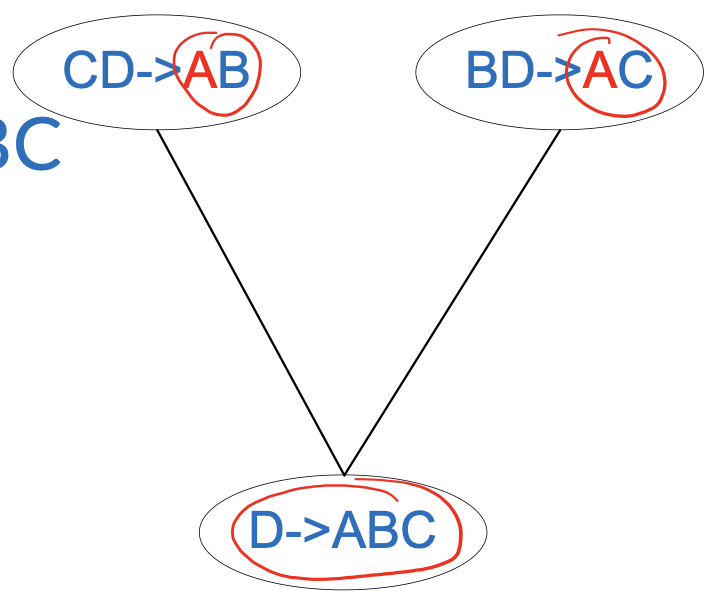
\includegraphics[width=1]{images/joining.png}
        \end{center}
    
    \subsection{FP-Tree and FP-Growth}
        The FP-tree contains a compressed representation of the transaction database. A trie \emph{prefix tree} data structure is used. Each transaction is a path in the tree. Paths may overlap.
        
        Once the FP-tree is constructed. We use the recursive divide-and-conquer FP Growth algorithm is used to enumerate all frequent itemsets. We order all the itemsets so we can define prefixes.
        
    \subsubsection{FP-Tree construction}
        Each path in the tree contains an itemset. We include the support on each vertex. Each vertex with a label contains pointers to all vertices with the same label. 
        
        \begin{center}
            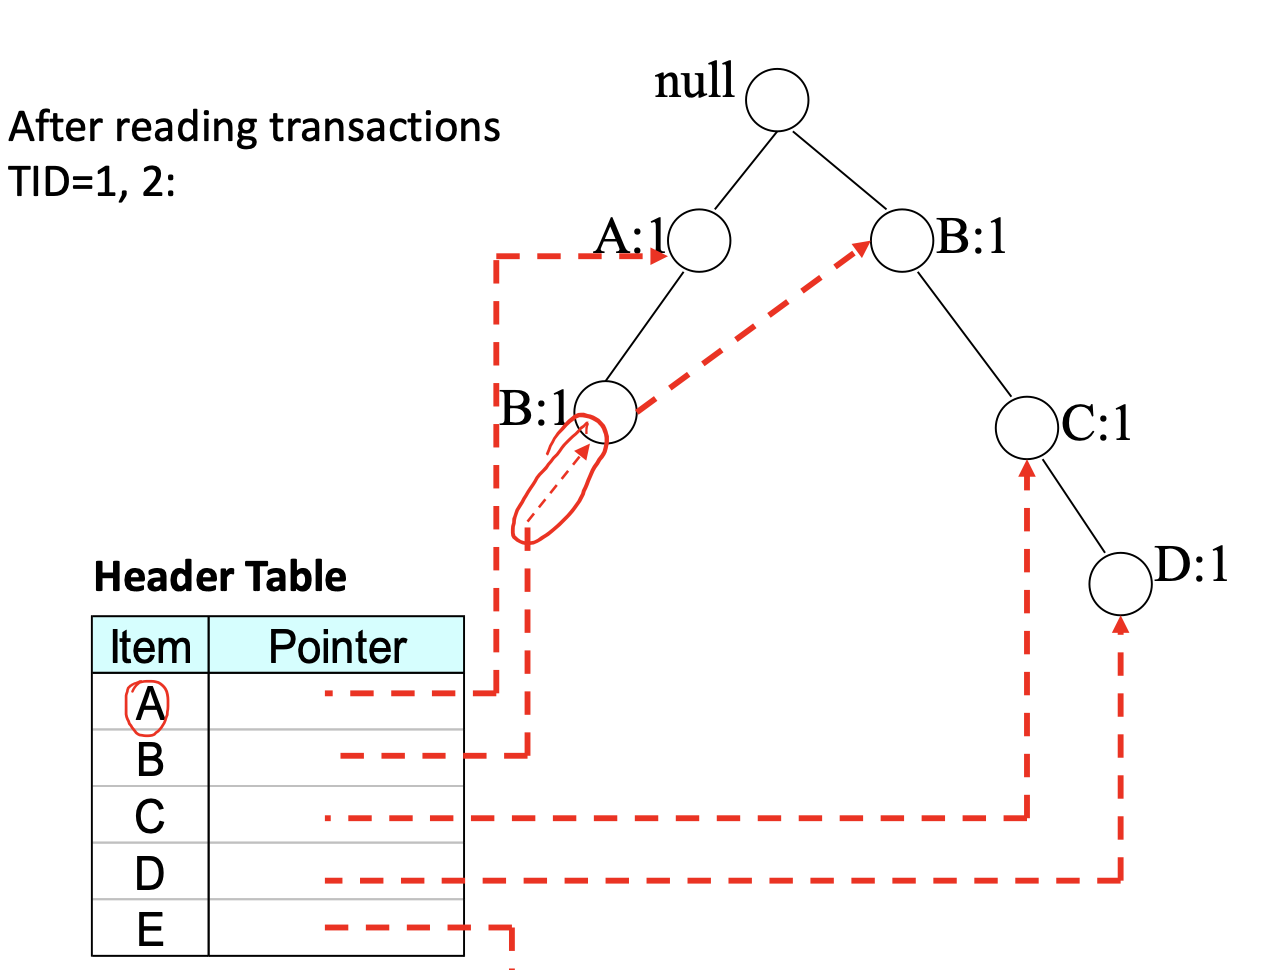
\includegraphics[width=0.7\textwidth]{images/fpconstruction.png}
        \end{center}
        
        Tree size depends on data compressibility. Tree size also depends on the ordering of items. We order items by frequency, from larger to smaller. 
        
           \begin{center}
            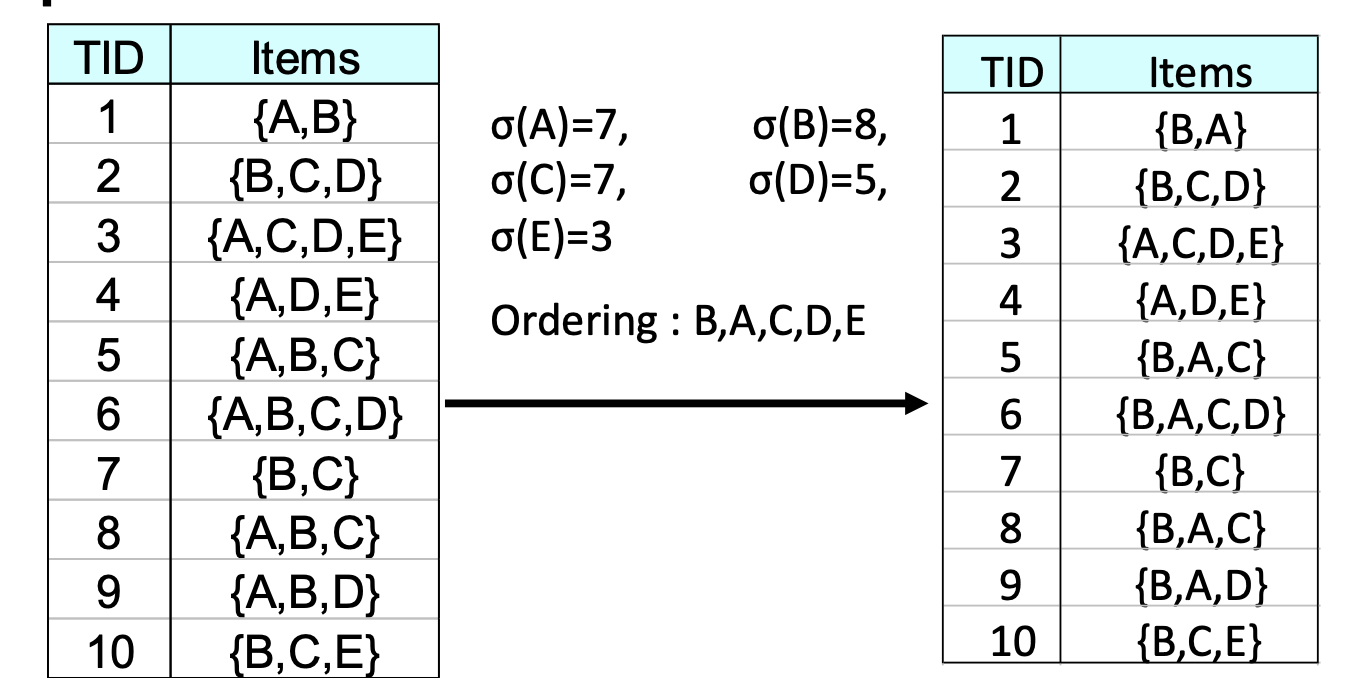
\includegraphics[width=0.7\textwidth]{images/ordering.png}
        \end{center}
        
    \subsubsection{Mining frequent itemsets on FP trees}
        Our algorithm takes as input an FP-Tree. It outputs all frequent itemsets and their supports. We will use divide and conquer.
        
        For each possible last item, consider itemsets with last items one of items preceding it in the ordering. E.g for E, consider all itemsets with last item $D, C; B, A$, this way we get all itemsets ending at $DE, Ce, Be, AE$. Proceed recursively this way. Do this for all items.
    
        \begin{center}
            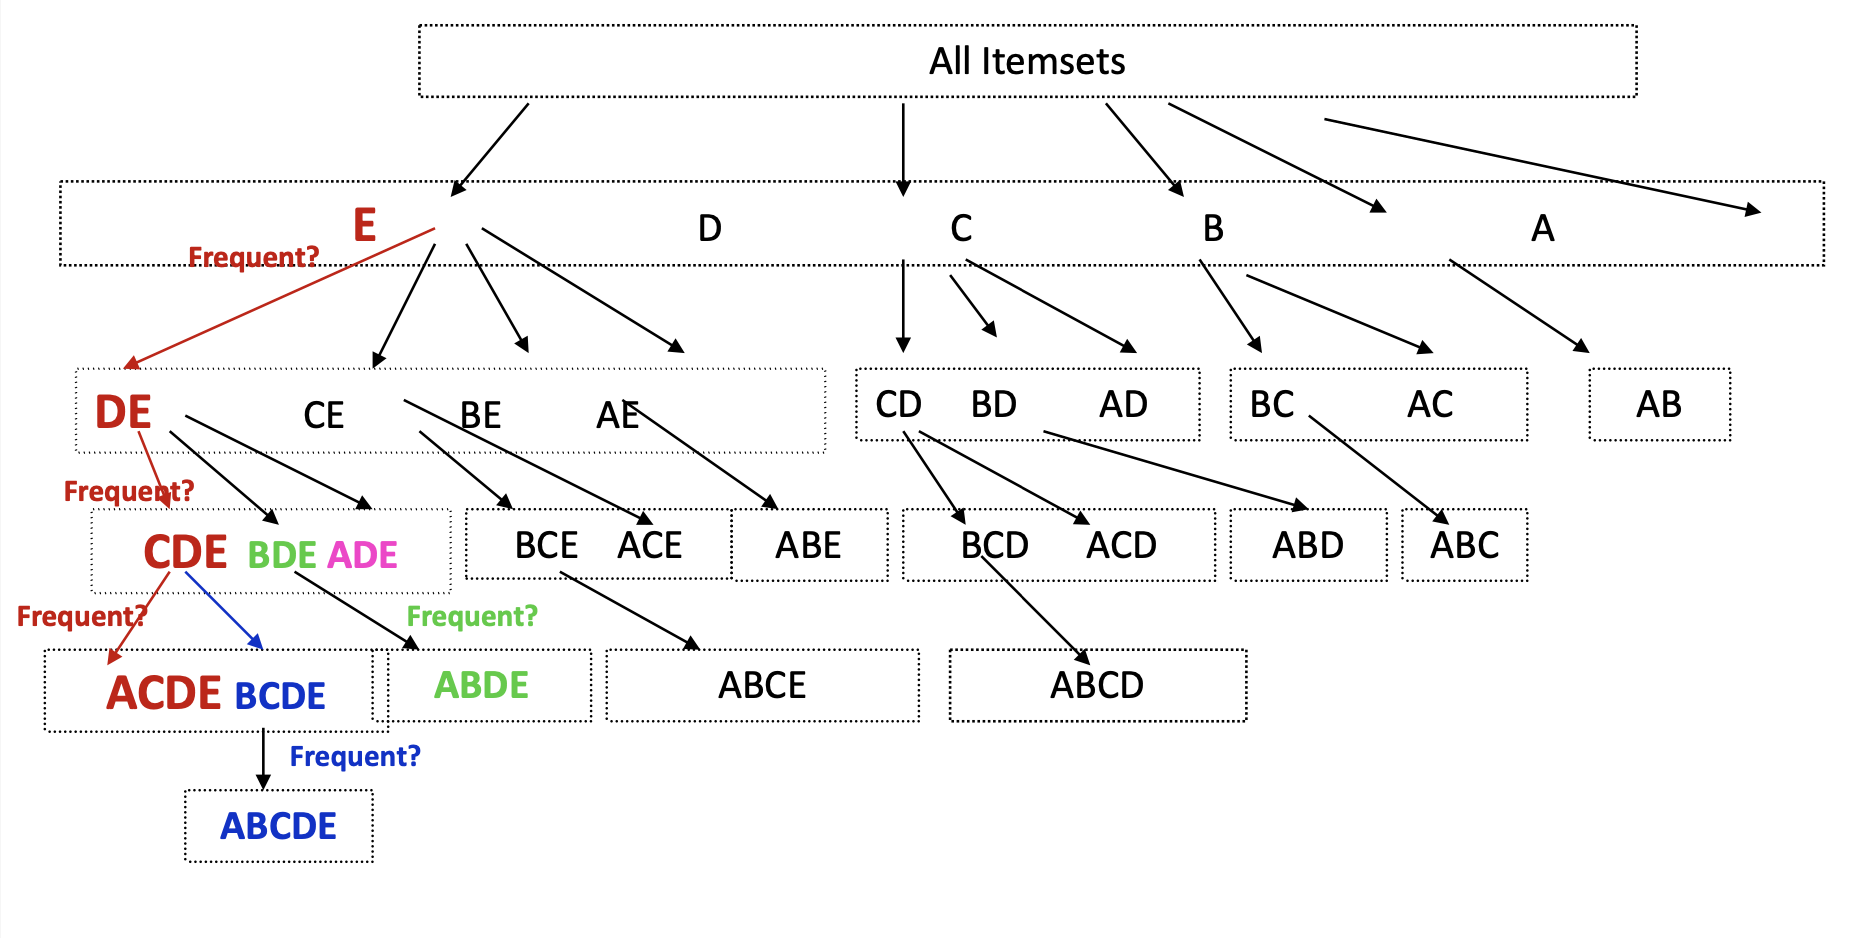
\includegraphics[width=0.7\textwidth]{images/miningfp.png}
        \end{center}
        
        This is basically a bottom-up traversal. We basically find all itemsets ending in the last one. 
        
        The algorithm works as follows
        \begin{itemize}
            \item For each suffix $X$, go to phase 1
            \item \textbf{Phase 1}: Construct a prefix tree for $X$, compute support using header table and pointers
            \item \textbf{Phase 2:} If $X$ is frequent, construct conditional FP-Tree \footnote{Elaborate conditional FP Tree} for $X$ in the following steps: \begin{itemize}
                \item Recompute support
                \item Prune infrequent items
                \item Prune leaves and recurse
            \end{itemize}
        \end{itemize}
        
        Observe that at each recursive step, we solve a subproblem of constructing the prefix tree, computing new support and pruning nodes. Subproblems are disjoint, so we never consider the same itemset twice. Support computation is efficient, happens along with computation of the frequent itemsets. Efficiency depends on how compressed the tree is.